\documentclass[12pt, letterpaper]{article}

\usepackage{amsmath} %% Allows for mathematical expressions such as binomials.
\usepackage{color} %% Allows text to be typeset in color.
\usepackage{amssymb}

%% These allow Me to add Images to the Book.
\usepackage{graphicx}
\graphicspath{ {images/} }

%% Enables hyperlinks.
\usepackage{hyperref}


% Typeset Algorithms.
\usepackage[subsubsection]{algorithm}
\usepackage{algorithmic}

% Allows for text with strikethroughs.
\usepackage[normalem]{ulem}

% Make the Captions small and italicized.
\usepackage[font={small,it}]{caption}

% Allows double spacing commands, such as \doublespacing.
\usepackage{setspace}

%% Makes BigO easier.
\newcommand{\bigO}{\mathcal{O}}
\newcommand{\bigOmega}{\Omega}
\newcommand{\bigTheta}{\Theta}

%% Redefines the varnothing symbol as the symbol for an empty set.
\let\emptyset\varnothing

%%
\oddsidemargin0cm
\evensidemargin0cm
\topmargin-2cm     % These lines increase the amount of usable space and save trees.
\textwidth16.5cm
\textheight23.5cm

%%\setcounter{tocdepth}{4} %% set the table of contents detail depth.

%% Types of organizational sections.s
%%\part{}
%%\chapter{}
%%\section{}
%%\subsection{}
%%\subsubsection{}
%%\paragraph{}
%%\subparagraph{}


\begin{document}

\pagenumbering{roman}
\doublespacing

\title{\color{blue}Extracting Curves from Subdivision Surfaces}
\author{Senior Honors Thesis by Bryce Summers \\
Carnegie Mellon University\\
Advisor: Keenan Crane}
\date{\color{red}Last Updated: \today}
\maketitle



\newpage

\section*{Abstract}
\addcontentsline{toc}{section}{Abstract}

	Effective communication of technical ideas often demands compelling mathematical diagrams and visualizations. 
	Just as TeX makes the best practices of professional mathematical typesetters accessible to everyday users,
	we aim to codify and automate best practices of professional mathematical illustrators.
	Currently, however, there is a functionality gap between 3D modeling software and 2D illustration software.
	The former allows users to manipulate 3D geometric information, while the latter allows users to manipulate aesthetic and stylistic information.

	We have begun the journey of reconciling these two software paradigms by developing essential algorithms for such a system. More concretly, we are 			studying the conversion of 3D Catmull Clark subdivision surfaces to 2D curve representations that are amenable to traditional aesthetic design and 			communicate the visual geometric relationships present in views of the 3D representation.

	// FIXME: Maybe I should mention traditional mathematical illustration.

\newpage

\section*{Acknowledgments}
\addcontentsline{toc}{section}{Acknowledgments}
\singlespacing

I would like to thank the people who have helped enrich my experience at Carnegie Mellon University (CMU),
which has led me to the ictus of completing this thesis, including those named explicitly here  and
those implicitly named in spirit who may efficiently know they are included in the geometric representation of my life.

CMU's Undergraduate Research Office (URO) afforded me my first opportunity to do research through in the form of a
Summer Undergraduate Research Fellowship (SURF), where I created the Summers Computer Aided Mathematics Program (CAMP).
I am very thankful for the help of the leaders of the URO at that time including \textbf{Jennifer Keating-Miller} and \textbf{Stephanie Wallach}
who helped me write my proposal and provided opportunities for me, as well as David Kosbie who advised me throughout the project.

As for my journey of playing around with beautiful geometry, I would like to thank \textbf{Nancy Pollard} for introducing me to subdivision surfaces,
\textbf{Golan Levin} for allowing me to write a subdivision algorithm for him during a time when I was discouraged,
and \textbf{Kayvon Fatahalian} for providing me with a second chance in my love affair with pedegogical computer graphics.

Finally I would like to especially thank my thesis advisor \textbf{Keenan Crane} who has
rekindled my intellectual curiosity by guiding my thoughts to new fields, knowledge, and modes of expression that I was previously unaware of.
He has been very patient with me, tolerated some of my more idiosyncratic ideas such as the study of the geometry of butter flowing through a popcorn field,
and maintained first class good humor during even the most difficult times.

I would like to thank the reasonable \textbf{Tom Cortina}, who I have enjoyed talking to over the course of my undergraduate experience, and who allowed me to 
participate in this Honors Thesis program, even though I missed the deadlines for the submission of the prospectus and this final
written document, which you are reading right now, due to extenuating circumstances.

Thank you to \textbf{Margaret Reid-Miller} and \textbf{Jacobo Carrasquel} for providing me with academic advice and lending my their perspectives.

Outside the direct realm of my computer science endeavors, I would like to thank \textbf{Helen Wang,
	Scott Sandage, Kunal Ghosh, John Mackey, Jarad Cohen, Lucas Christian},
and \textbf{R. James Whipple} for the friendship, empathy, and compassion that they have shown to me, my ideas, and my world view.

Thank you to all of my \textbf{collegiate peers} who I have learned to interact with, learn from, and appreciate.

For my final statement of acknowledgment, I would like to thank open minded parents \textbf{Bruce} and \textbf{Mary},
my wonderful sister \textbf{Katey}, and the rest of my \textbf{family} for remaining
invariant in their support of me through my non euclidean transformations. They therefore define a geometry on and beneath the surface of my life.


\newpage
%% The Location of the table of contents.
\doublespacing
\tableofcontents
\newpage

% Set up the formatting for the bulk of the document.
\setcounter{page}{1}
\pagenumbering{arabic}


\section{Introduction}

	Our work seeks to bridge a functionality gap between 3D Modelling software and 2D Illustration software. We will start out by describing each of these
	software paradigms along with their strengths and weaknesses. We will then describe our proposed synthesis of these two paradigms and related problems
	that must be addressed in the creation of this new software.


	\paragraph{3D Modeling Software.}

	Traditional 3D modeling software, such as the open source \emph{Blender} program, are used primarily for defining the geometry and visual appearance of models to be 
	used in various applications such as 3D animation, the automative industry, and architectural visualization.
	These programs use the latest and greatest algorithms in the fields of computational geometry, rendering, and Computer Aided Design,
	but they do not have the capability to stylize their models with prescision. Many of them are geared towards rendering the models using 
	realistic models of light transport. As discussed in \cite{JDA08}, realisitic lighting is not necessarily the best stylistic descision for communicating
	geometric information about an object. See \ref{fig:photorealistic_rendering} for an example realistically rendered image.
	Please see \ref{fig:keenan_cow} for a typical 3D model as might be seen during manipulation in a 3D Modeling program. The visual style communicates
	the individual discrete vertices, edges, and faces that a user can modify which is important to a person constructing a 3D model, but it does not
	emphasize visual information that would be important to a geometer or a person concerned with aesthetics.

	\begin{figure}[h]
	\centering
	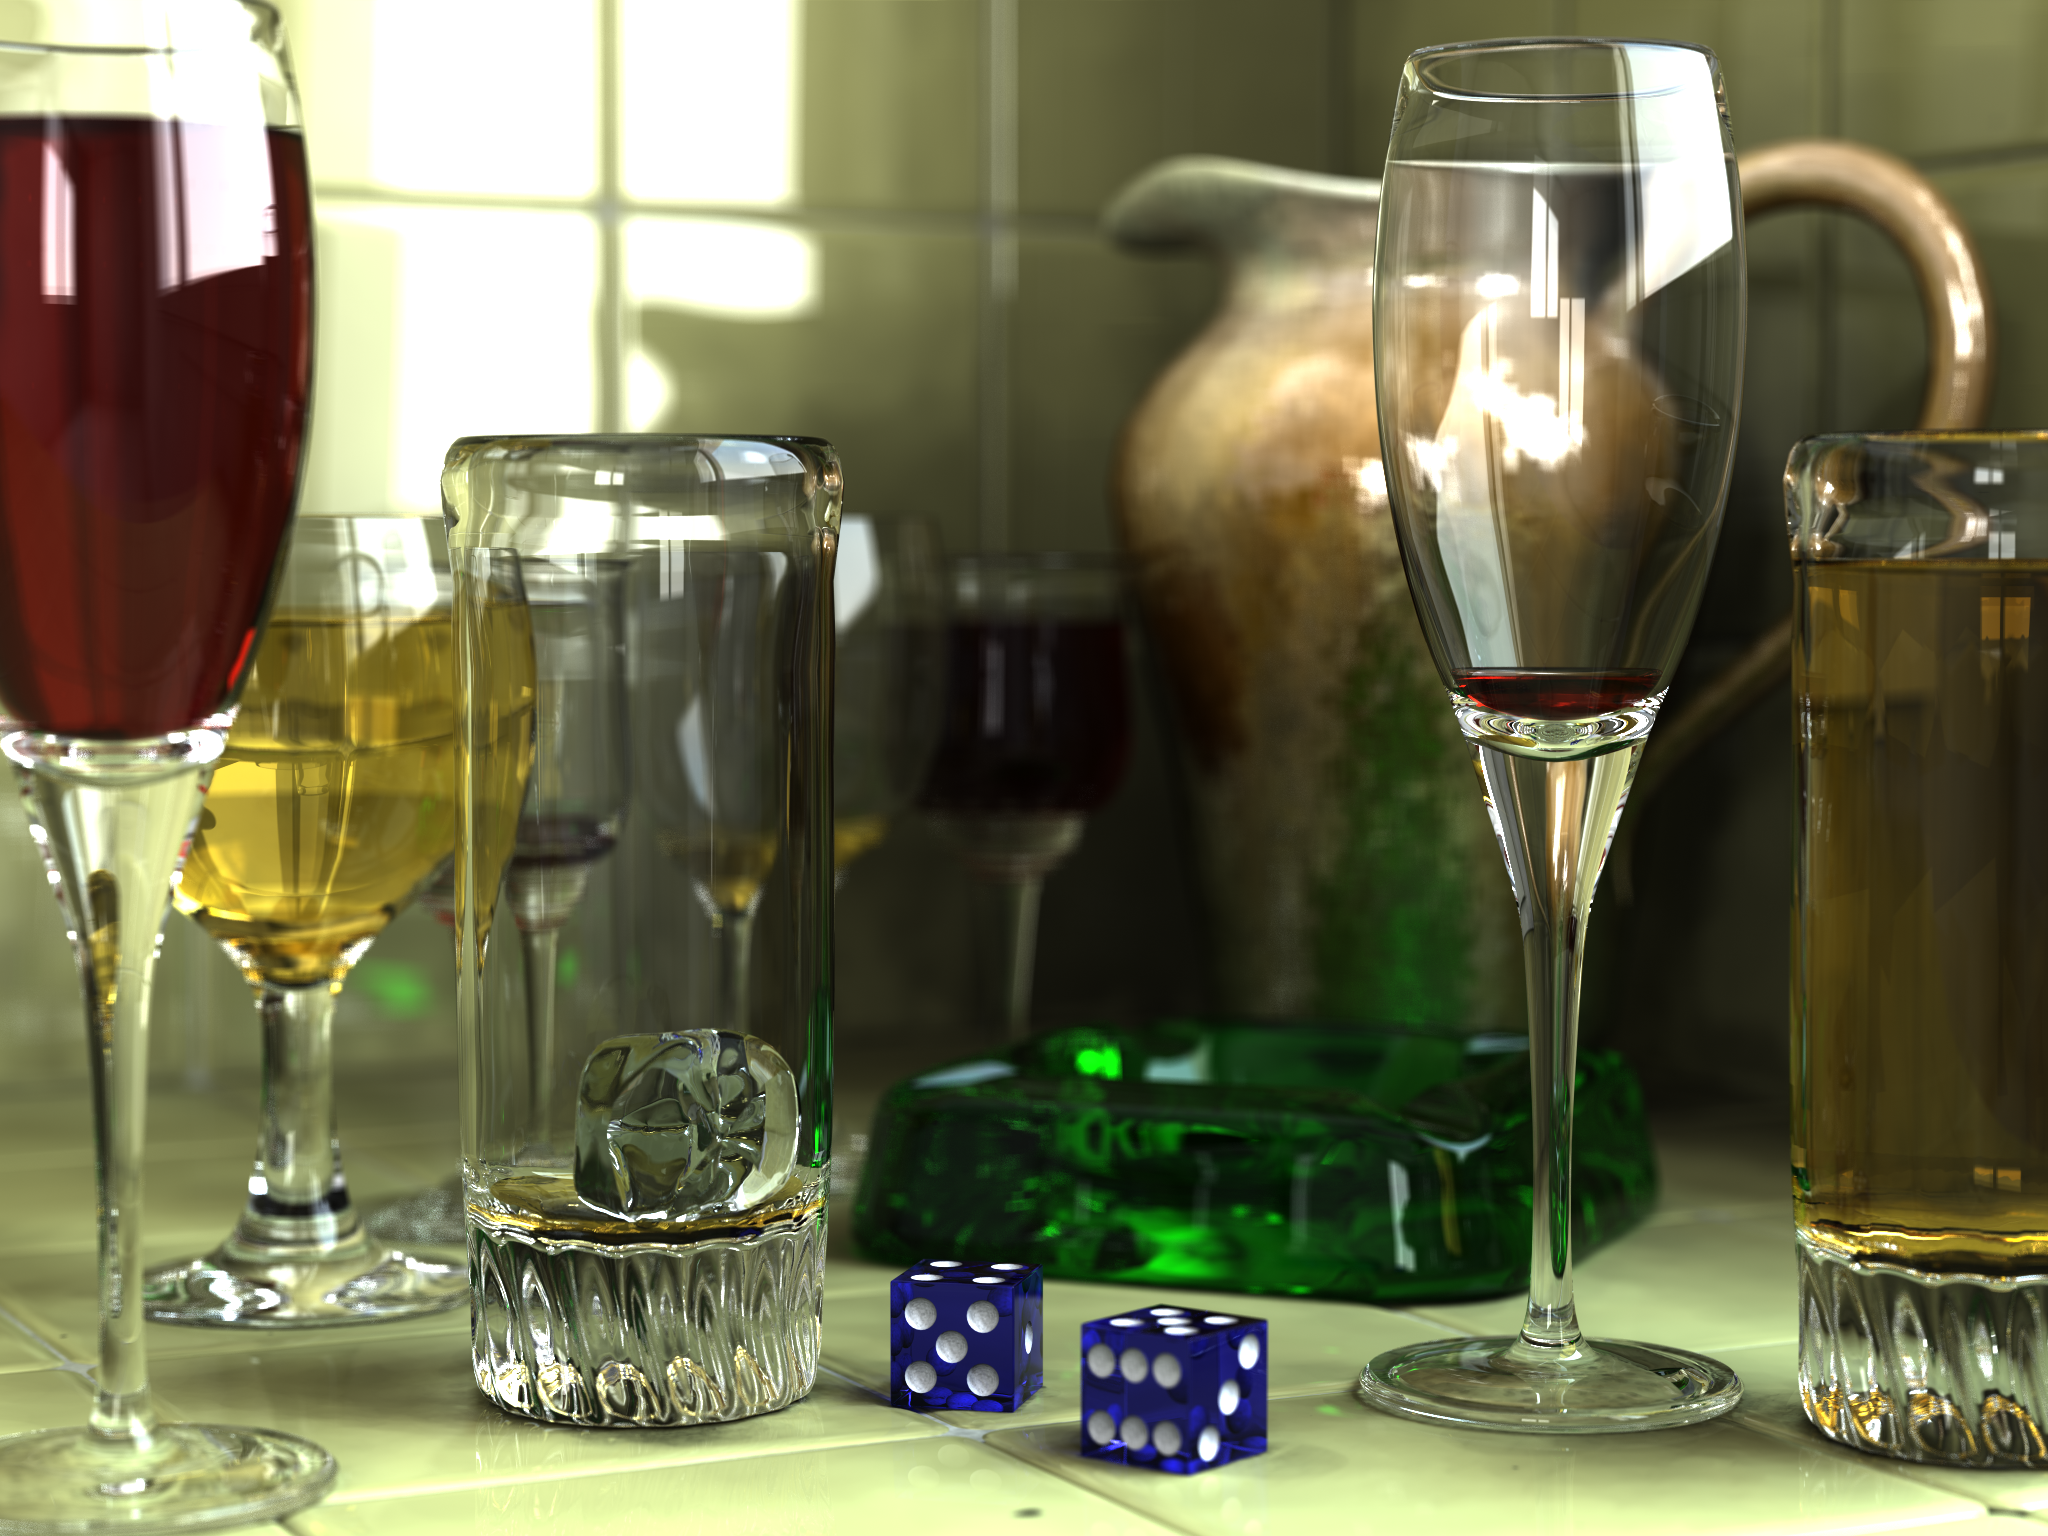
\includegraphics[width=0.5\textwidth]{PhotorealisticRendering}
	\caption{3D modeling systems are often used to produce photorealistic imagery, which is not always the proper best at communicating geometric information as discussed in \cite{JDA08}.
		Notice how difficult it is to discern the edges and faces of the dice,
		how the reflections of the bright light from the window obscure the structure of the glasses, and the shadows make it hard to read the visual extent of the glass hidden in the dark background.
		Image Credit: Gilles Tran on Wikipedia.}
	\label{fig:photorealistic_rendering}
	\end{figure}

	\paragraph{2D Illustration Software.}

	2D illustration software, such as the open source \emph{Inkscape}, are used primarily by designers and communicators to create 2D svg illustrations that
	communicate ideas, rather than realistic visual artifacts. They have a lot of capabilties for modifying the colors and stroke sizes of lines and interiors,
	labeling important features with textual boxes and arrows, and compositing different visual objects on top of each other through blending.
	While they are great at manipulating the aestetics of images, they do not necessarily understand 3D geometry and take it into account in the manipulations
	that they support. Please see Figure: \ref{fig:cornell_box_illustration}, which is an example 2D illustration that we created in \emph{Inkscape} that communicates light transport within a traditional Cornell Box scene.

	\begin{figure}[h]
	\centering
	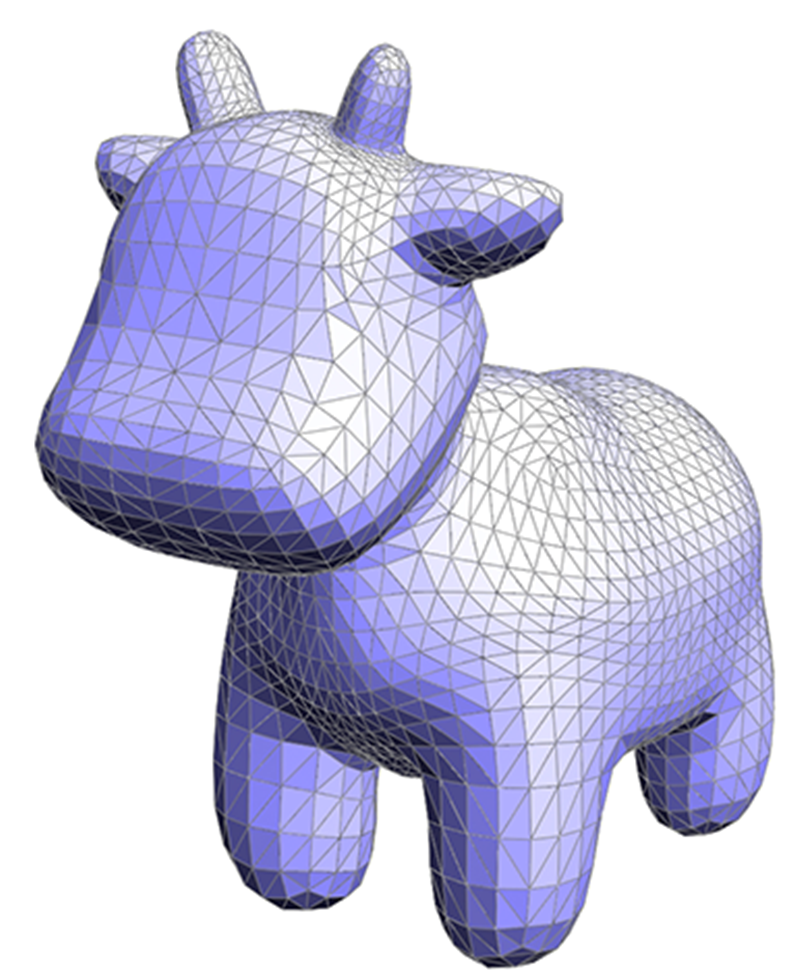
\includegraphics[width=0.3\textwidth]{KeenanCow}
	\caption{A typical 3D model that is manipulated in a 3D modeling program. Note the visual emphasis on representational features associated
			with the discretization of the geometry such as the triangular faces and flat shading, rather than the emphasis on light transport properties emphasized
			in realistic renderings like in Figure: \ref{fig:photorealistic_rendering} or the continuous geometric properties emphasized in our desired system such
			as in Figure: \ref{fig:keenan_style}}.
	\label{fig:keenan_cow}
	\end{figure}

	\paragraph{Geometric Latex.}

	Our goal is to unify these two paradigms to enable the creation of figures that are generated directly from 3D geometric mathematical models 
	and amenable to stylistic modification that takes advatage of the geometric information. In essense, we wish to create a ``geometric \LaTeX" program.
	See Figure: \ref{fig:keenan_style} for an example illustration that
	we could make natively using such a program. We would also be able to easily produce traditional mathematical illustrations such as those found in 
	Tristan Needham's book, \emph{Visual Complex Analysis}. Most high quality mathematical illustrations found in the literature are hand drawn,
	but through out work people should eventually find it easier to create high quality geometric illustrations using software in lieu of non digital methods.

	\begin{figure}[h]
	\centering
	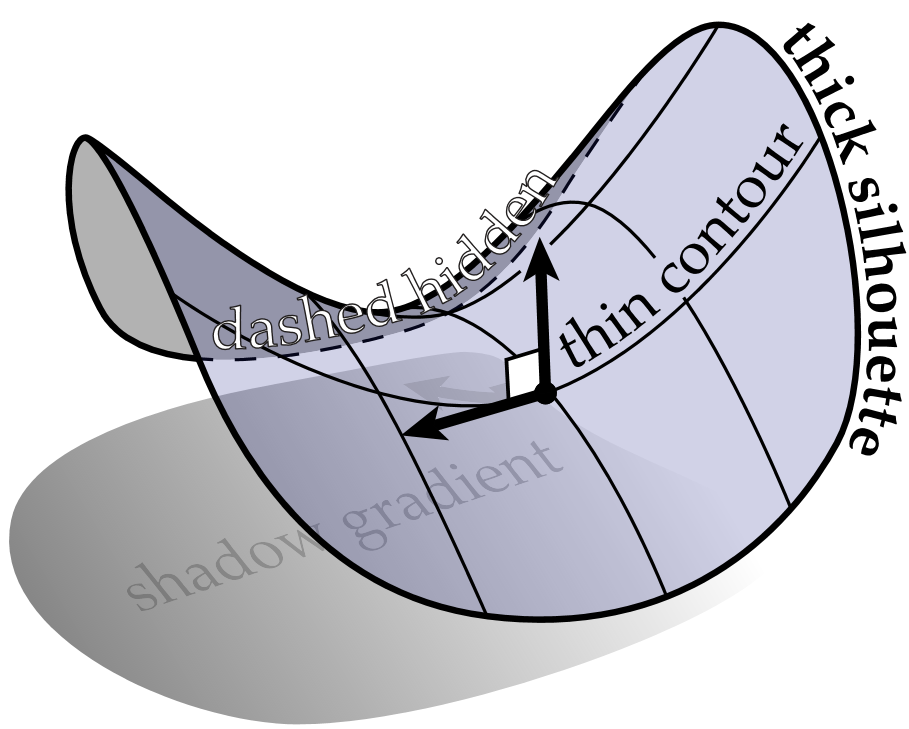
\includegraphics[width=0.4\textwidth]{StylizedFigure}
	\caption{A 3D geometric image created with proper aesthetic design. To create this image, a system would need to model the saddle geometry along
	with its smooth boundary, compute tangents and curvatures,
	extract minimum and maximum curvature curves to defined the local coordinate system, extract smooth silhouette curves, segment curves based on occlusion,
	extract the planar shadow via a silhouette curve projection, and provide user features for curve and tangent aware labels.
	The system would need to be able create gaps at intersections between labels, arrows, and the geometric curves.
	The Image is Courtesy of Keenan Crane.}
	\label{fig:keenan_style}
	\end{figure}

\newpage

	\paragraph{Foundational Problems}
	To realize the goal of a geometric \LaTeX program, we need to solve many problems revolving around the extraction of important curves from 3D models
	such as those used for stylization in Figure \ref{fig:keenan_style}. In general, we need to develop algorithms for extracting representations for any curves
	that communicate important visual or geometric information or that may be required for the conversion between the processes defined within each paradigm
	that are not yet compatible with each other, such as fills in 2D and shadow casting in 3D. In particular, we have investigated the extraction of silhouette curves and parameter curves,
	as well as critical points and integral curves for the Morse-Smale complex. We have also investigated various sub problems for curve extraction,
	including locating \emph{every} curve, finding unique representative points for every curve, gradient descent methods, and planar curve projections.

\newpage

\section{Background/Prior Work}

	\subsection{Important 2D curves for projected 3D models.}

		Various curves on surfaces communicate important geometric information. Here is a list of some relevant curves that folks have
		tried to extract from surfaces in the past.

\begin{itemize}
	\item 	\textbf{Parameter curves} are useful in showing lines along a collection of quadrilaterals and showing global coordinate systems.
			They are useful primarily because 3D models are often created using a discretization that follows the symmetries and geometric structure
			of the object they are modelling.
	\item 	\textbf{Silhouette curves} communicate the visual extent of the model and the boundary.
			The projection of silhouette curves onto a plane determine the shadows that a surface casts.
			The collection of silhouette curves for a surface without double negative curvature defined with regards to every viewing direction constrained to a plane
			is sufficient to describe the geometry of the surface.
	\item 	\textbf{Minimum - Maximum curvature curves} communicate the curvature of the model and locally intuitive coordinate systems.
	\item        \textbf{Geodesic curves} communicate the path on the surface of minimum distance between two points on a surface.
	\item 	\textbf{Integral Lines}: lines that follow the gradient of a function defined on a surface from one critical point to another. These may be used to form the Morse-Smale complex
			which segments the model into regions with similar monotonic functional behavior.
\end{itemize}

	\subsection{Previous Extraction Methods}

	\paragraph{2D Curve Extraction Methods.}

		Many people have extracted silhouette curves by simply tracing the exterior boundary of a 2D rasterization of the surface. This approach suffers from 
		discretization and sampling problems and does not provide much information about the 3D geometric structure of the silhouette curves.
		For instance, they can't be used to compute direct shadows.
		It also may be possible to extract silhouette curves using an algorithm akin to the marching squares, but again it would suffer from the same sorts of problems.
	
	\paragraph{3D Curve Extraction Methods.}

	Stroila et. al. were able to extract silhouette, shadow, gleam, and other curves via particle chain systems. They have also studied practical ways to utilize these curves
	for illustration by describing how to sort, orient, identify, and fill them as closed regions. \cite{SEH08} // FIXME: Should I rephrase this, because 
	I am pretty much parroting the abstract of this paper.

	\subsection{Catmull-Clark Subdivision Surfaces}
	
	// FIXME : I need to define what Catmull-Clark Subdivision Surfaces are.

		Naively we could directly evaluate these curves over the linear patches defined on standard polyhedral 3D models,
		but much like the results found in \cite{Eisemann08},
		such lines would jitter back and forth over boundaries and would not converge to smooth natural and correct looking curves even after substantial
		subdivision of the surface. See Figure \ref{fig:Eisemann_linear_patches} for example of Eisemann et Al's attempt to extract silhouette
		curves from linear patches. We therefore wish to work on Catmull-Clark Subdivision surfaces that allow us to take a discrete quadrilateral control mesh
		and perform calculations on its limit defined subdivision surface, instead of any intermediate discrete representation.
		See Figure : \ref{fig:subDDef} for an illustration of control meshes and limit surfaces.

		\begin{figure}[h]
		\centering
		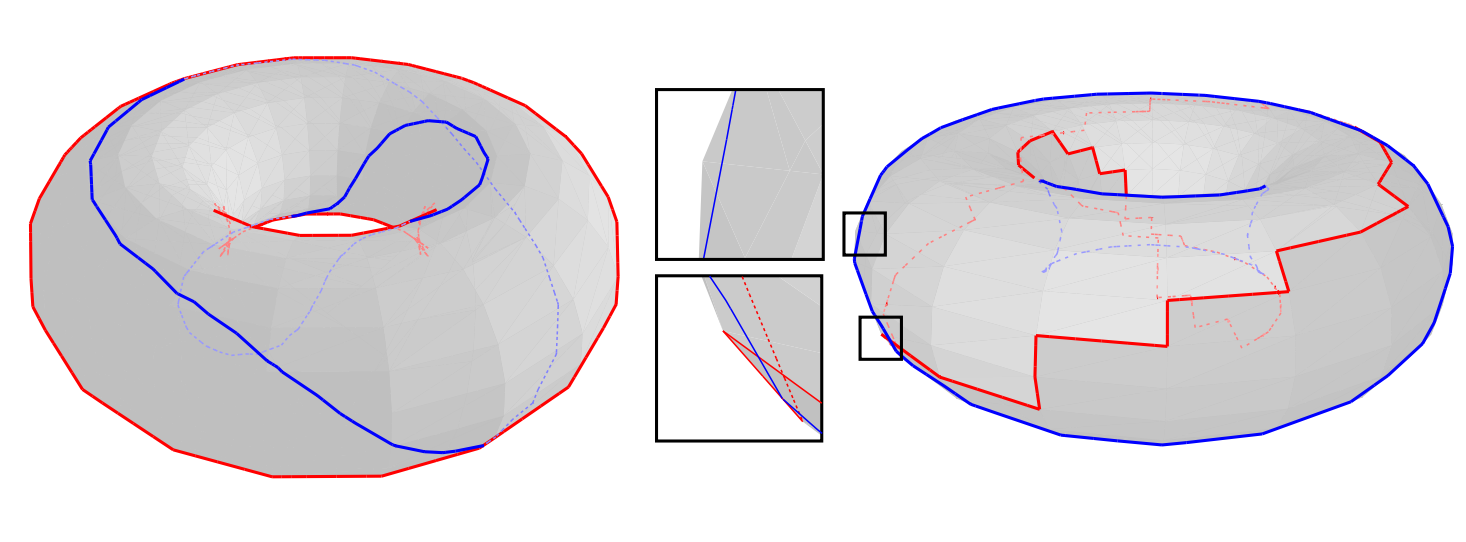
\includegraphics[width=0.5\textwidth]{Eisemann08_linear_patches}
		\caption{Linear Patches Silhouette curves either produce staircase patterns or don't properly lie on the geometry, even in the limit. Image Credit: \cite{Eisemann08}.}
		\label{fig:Eisemann_linear_patches}
		\end{figure}

		\begin{figure}[h]
		\centering
		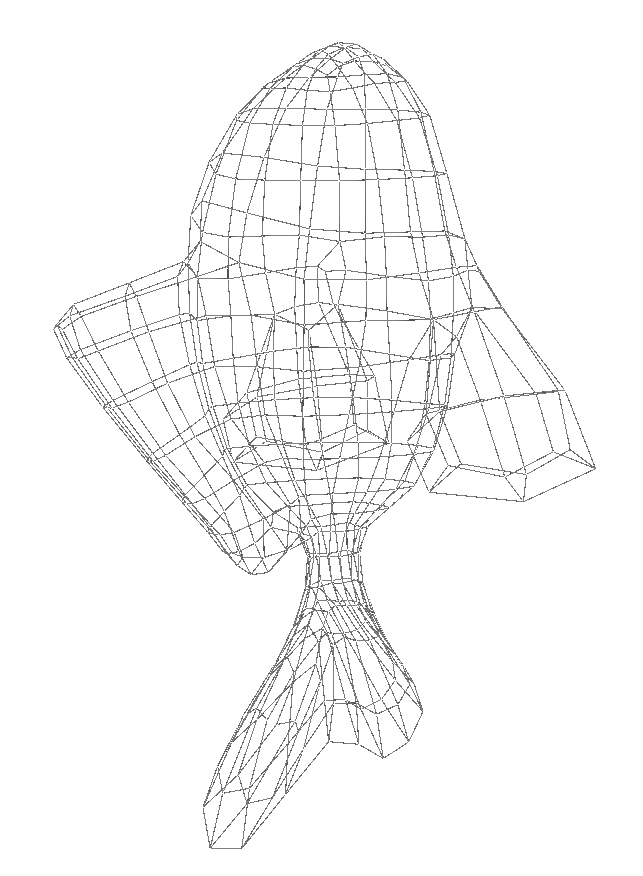
\includegraphics[width=0.3\textwidth]{fish_cm}
		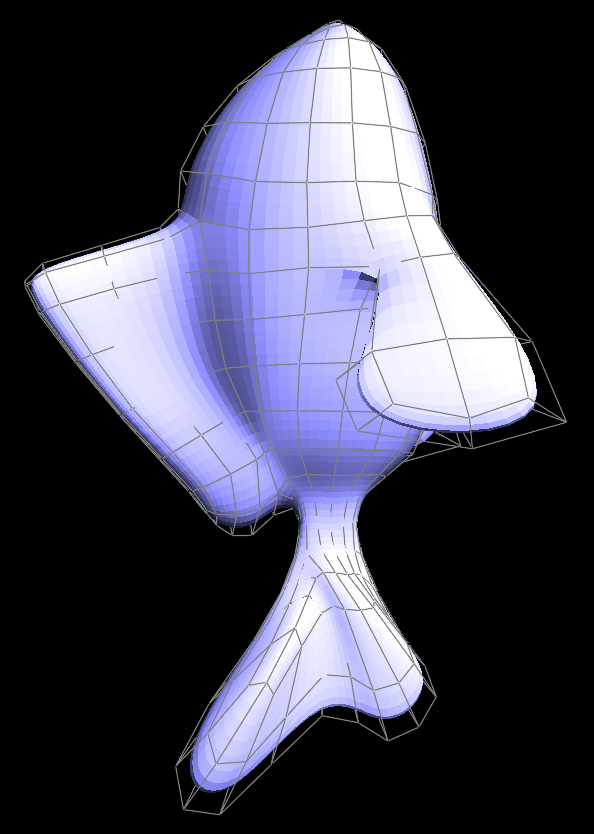
\includegraphics[width=0.3\textwidth]{fish_cm_and_patch}
		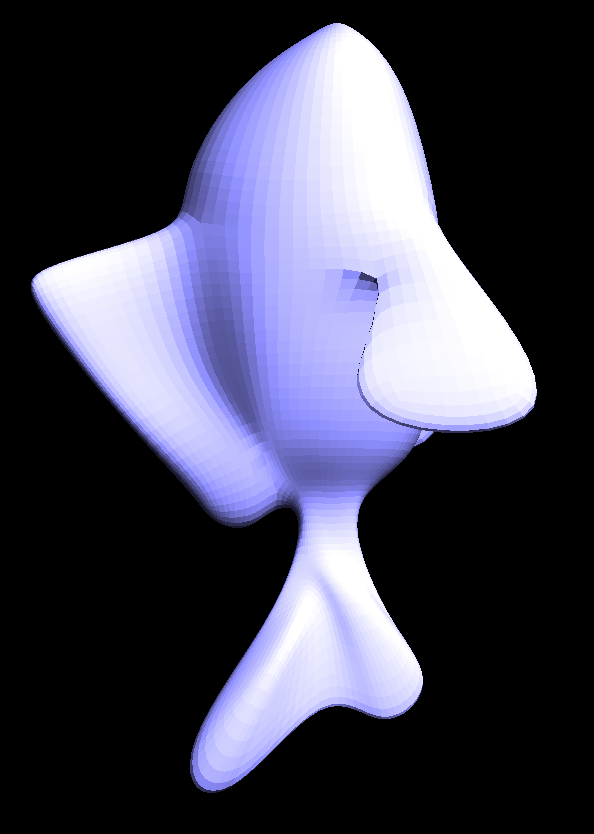
\includegraphics[width=0.275\textwidth]{fish_patch}
		\caption{A model of a fish represented from on the left by its control mesh and on the right by a geometry patch approximation of its Catmull-Clark limit surface.}
		\label{fig:subDDef}
		\end{figure}

	\newpage

	\subsection{Loop - Shaeffer Approximations}
	
		No matter how finely we refine a traditional Catmull-Clark surface, it will still be a collection of linear patches which suffer from the same problems as 
		in \cite{Eisemann08}.  We therefore get around this problem by directly computing a continuous and differentiable approximation of the limit surface
		via the scheme described in \cite{Loop}
		We can create a one-to-one correspondence between faces in the control mesh and bicubic bezier surfaces (a.k.a ``patches") that approximate the 
		limit Catmull-Clark subdivision surface that the faces represent.
		To do so, we follow the procedure outlined in \cite{Loop}.
		We therefore are able to derive control points for a geometry patch which we will denote $G_{ij}$ (Figure: \ref{fig:G}) and two tangent patches, 
		one for each principal parameter direction along the bicubic patch (Figure: \ref{fig:dU} and Figure: \ref{fig:dV}).
		The tangent patches are necessary, because the geometry patches only exhibit G0 continuity in the presense of extraordinary vertices. Roughly speaking, this means that the neighboring geometry patch boundaries having matching positions, but different tangent vectors.
		Since any quadrilateral mesh that is not homeomorphic to a torus must contain an extraordinary vertex,
		it is essential that we use the tangent patches to ensure effective differentiability everywhere along the surface formed by the union of the bicubic patches.
		
		For the remainder of the paper, we will be using these Loop - Schaeffer patch defined surfaces defined on quadrilateral meshes and refer to them simply as ``surfaces".
		We will assume that these surfaces do not contain boundaries.

		\begin{figure}[h]
		\centering
		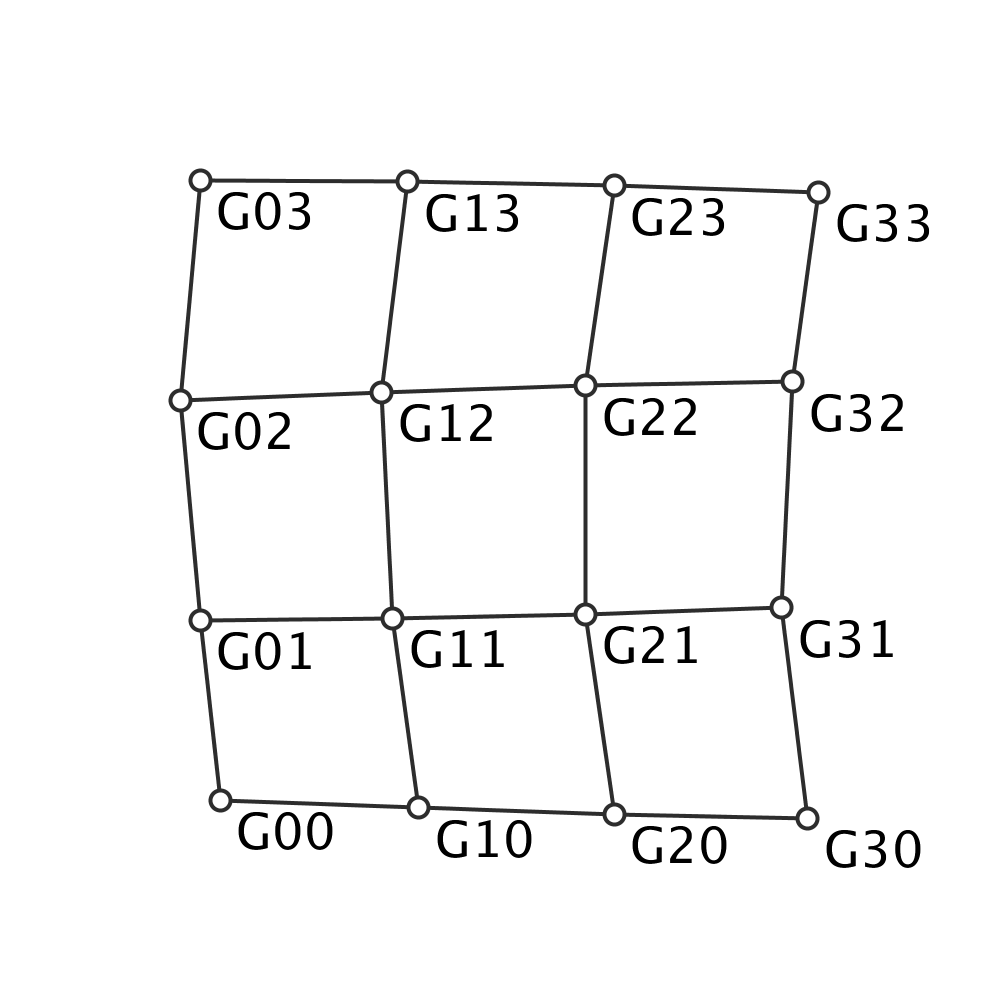
\includegraphics[width=0.35\textwidth]{GeometryPatchControlPoints}
		\caption{Geometry Patch Control Points for a single control mesh face.}
		\label{fig:G}
		\end{figure}

		\begin{figure}[h]
		\centering
		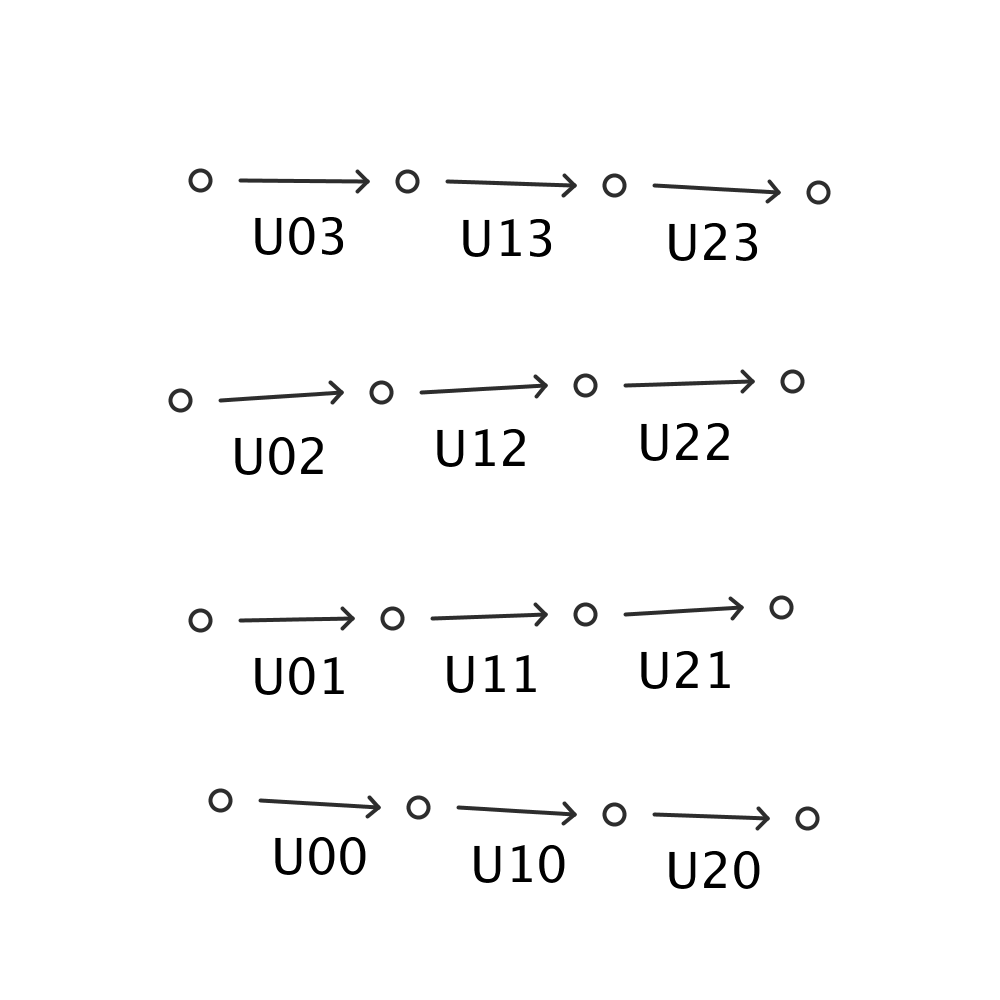
\includegraphics[width=0.35\textwidth]{duPatch}
		\caption{$\partial u$ tangent patch control vectors for a single control mesh face.}
		\label{fig:dU}
		\end{figure}

		\begin{figure}[h]
		\centering
		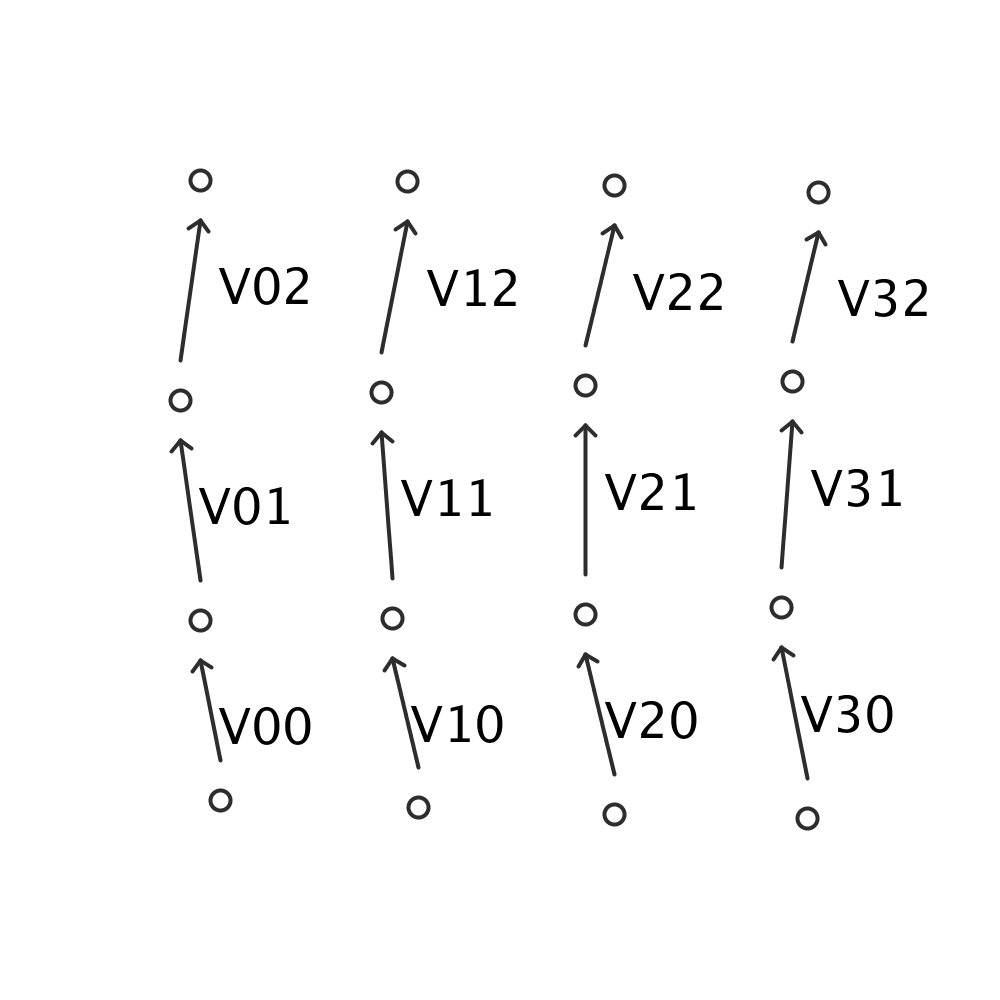
\includegraphics[width=0.35\textwidth]{dvPatch}
		\caption{$\partial v$ tangent patch control vectors for a single control mesh face.}
		\label{fig:dV}
		\end{figure}



\section{Methodology}

	\subsection{Definitions and Calculus on Bicubic Patches}
	
	In this section we will discuss some fundamental calculus computations involving the patches that will be used in curve extraction algorithms.

		\paragraph{Bezier Surfaces}
		A \emph{bicubic patch} is a \emph{bezier surface} that can be represented explicitly in terms of the so-called
		\emph{Bernstein polynomials}, and interpolates data points.
		The beauty of the bicubic patch approximations for Catmull-Clark subdivision surfaces described by Loop and Schaeffer
		is that they allow us to transition from discrete math to well defined continuous math.

		The Bernstein polynomials are defined as follows:

		$$\mathcal{B}_{i, n}(x) = \mathcal{B}_{i}^{n}(x) = \binom{n}{i}x^{i}(1-x)^{n-i} \; \textbf{for} \; i \in \{0, \cdots, n\}  $$
		
		Two-dimensional Bezier surfaces are defined parametrically as follows: 
		
		$$[0, 1] \times [0, 1] \rightarrow \mathbb{R}^{3} : \sum_{i=0}^{n}{\sum_{j=0}^{m}{\mathcal{B}_{i}^{n}(u) \mathcal{B}_{j}^{m}(v) C_{i, j}}}$$
		
		where $n, m$ is the degree of the surface, which is represented by $(n + 1) \cdot (m + 1)$ control points denoted genarically here by $C_{ij}$.
		
		\paragraph{Geometry Patches}

		The geometry patch surfaces are of degree (3, 3) and are therefore represented by the 16 control points $G_{ij}$ as follows:
		
		$$g(u, v) = \sum_{i=0}^{3}{\sum_{j=0}^{3}{\mathcal{B}_{i}^{3}(u) \mathcal{B}_{j}^{3}(v) G_{i, j}}}$$
		
		\paragraph{Partials Defined by Geometry Patches}

		We can easily take partial derivatives of a Geometry Patch as follows:

		$$g_{u^{m}v^{n}} = \frac{\partial g}{\partial u^{m} \partial v^{n}} = \sum_{i=0}^{3}{\sum_{j=0}^{2}{\mathcal{B}_{i, 3}^{(m)}(u) \mathcal{B}_{j, 3}^{(n)}(v) G_{i, j}}}$$

		where $m$ and $n$ are the degrees of differentiation in $u$ and $v$ respectively.

		\paragraph{Partials Defined by Tangent Patches}
		
		We can easily take partials of $g$ in $u$ and $v$ by differentiating the relevant $u$ or $v$ parameterized bezier function,
		but for the most part we will not make use of this pleasantry, because the geometry patches may be non differentiable on the boundaries.
		We will instead evaluate the partials from the tangent patches.
		
		\begin{equation} \label{eq:g_u}
		g_{u} := \frac{\partial g}{\partial u} = \sum_{i=0}^{3}{\sum_{j=0}^{2}{\mathcal{B}_{i}^{3}(u) \mathcal{B}_{j}^{2}(v) U_{i, j}}}
		\end{equation}

		\begin{equation} \label{eq:g_v}
		g_{v} := \frac{\partial g}{\partial v} = \sum_{i=0}^{2}{\sum_{j=0}^{3}{\mathcal{B}_{i}^{2}(u) \mathcal{B}_{j}^{3}(v) V_{i, j}}}
		\end{equation}

		\paragraph{Normals}

		The normal direction is defined for any point on the surfaces as follows:

		$$N(u,v) = g_{u} \times g_{v} (u, v)$$

		Typically normal vectors would be normalized to a unit length, but for the purpose of extracting silhouette curves
		this normalization will not effect the final results, which enables us to use the simplified (unnormalized) expression.
		Not only is the simplified expression easier to differentiate symbolically, it also outputs 3 dimensional vectors containing multinomials,
		which work well with the root finding algorithms in Section : \ref{section:rootFindingGeometryPatch}.
		
		\subsubsection{Gradient Descent}
		\label{section:GD}

		// FIXME : See about restating this further.
		
		Many of our algorithms rely on gradient descent to optimize various functions on surfaces. A proper selection of step sizes is important for these
		operations. If the steps are too slow, then performance will suffer due to slow convergance. If the steps are too large, then the optimization procedure may overshoot local minnima and fail to converge.
		Gradient descent on a function $f : \mathbb{R}^{n} \rightarrow \mathbb{R}$ :  requires that $f$ be differentiable. A direction $u \in \mathbb{R}^{n}$ 
		is a \emph{search direction} if the directional derivative of $f$ along $u$ is negative. In other words for a search direction $u$, the following holds:

		$$ D_{u}f = \nabla f \cdot u < 0$$

		Given an initial point $x_{0}$ and a search direction $u$, we want to find a new point $x_{1} := x_{0} + \tau u$ that is of a step size that is guranteed to make progress towards finding a local minnima. 
		The step size should therefore satisfy two conditions as follows:

		\begin{enumerate}
		\item The \textbf{Armijo condition} $f(x_{0} + \tau u) \le f(x_{0}) + c_{1} \tau D_{u} f(x_{0})$\\
		\item The \textbf{Wolfe condition} $|D_{u}f(x_{0} + \tau u)| \le c_{2}|D_{u}f(x_{0})|.$
		\end{enumerate}

		where $c_{1}, c_{2} \in \mathbb{R}$ are any two constants such that $$0 < c_{1} < c_{2} < 1.$$

		We can then compute the step size via the following algorithm: %% \ref{alg:step_size}

		\begin{algorithm}
%%		\caption{Given a surface, a point, and a fixed yet arbitrary u direction, this procedure computes the visible and nonvisible portions of an \textbf{axis aligned parameter curve}.}
		\label{alg:step_size}
		\begin{algorithmic}
			\STATE \textbf{begin}
			\STATE $\alpha \leftarrow 0$
			\STATE $\beta \leftarrow +\infty$
			\STATE $\tau \leftarrow 1$
			\REPEAT
				\IF{Armijo is not satisfied}
					\STATE $\beta \leftarrow \tau.$
				\ELSIF{Wolfe is not satisfied}
					\STATE $\alpha \leftarrow \tau$
				\ELSE 
					\STATE BREAK.
				\ENDIF
				\IF{ $\beta < +\infty$}
					\STATE $\tau \leftarrow (\alpha + \beta)/2$
				\ELSE
					\STATE $\tau \leftarrow 2 \alpha$
				\ENDIF
			\UNTIL{BREAK}
			\STATE \textbf{end}

		\end{algorithmic}
		\end{algorithm}

		For the purposes of this thesis, we will label gradient descent operations as follows:
		$$ x_{1} = \text{GD}(f, x_{0})$$ where $x_{0}$ is the initial point, $f$ is a differentiable function, and $x_{1}$ is the resultant minnimization of the function.
		
		\subsubsection{The Visibility Function}

		In the context of this thesis, we will define the \emph{visibility function} as a measure of
		whether the surface is forward or backward facing relative a viewing direction.
		Given a fixed yet arbitrary viewing direction $E$ we can define the \emph{visibility function} as follows:

		$$f(u, v) = N(u, v) \cdot E$$

		A location $(u, v)$ in parameter space on a surface is visible if and only if $f(u, v)$ is negative.
		Note that the location may still be occluded by another portion of the geometry.
		Also note that we are assuming an orthonormal viewing direction, instead of a perspective projection,
		because it simplifies our mathematics. \cite{XJY98}

		\paragraph{Silhouette Curves and Points}

		A Silhouette point $p$ is any point such that the visibility function is zero. In other words the following must hold:
		$$p = g(u, v) \textbf{ and } f(u, v) = 0$$

		A silhouette curve contains a closed ordered set of silhouette points. In other words they are defined as the boundary between the visible and non visible regions of the surface.

		\paragraph{Behavior of Visibility Function}

			Assuming that $E$ has unit length, the following properties hold for the visibility function:

			\begin{itemize}
			\item $f$ has a bounded range as follows: $-|N| \le f(u, v) \le |N|$
			\item $f$ has a Global Minimum when $f(u, v) = -|N|$.
			\item $f$ has a Global Maximum when $f(u, v) = |N|$.
			\item Silhouette curves are defined when $f(u, v) = 0$.
			\end{itemize}

		\paragraph{Partials of the Visibility Function}

			The first order partial derivatives for the visibility function may be derived as follows using applications of the product rule for derivatives of cross products:

			\begin{align*}
			N(u, v) &= g_{u} \times g_{v} (u, v)\\
			f  &= E \cdot (P_{u} \times P_{v})\\
			\frac{\partial f}{\partial u} = f_{u} &= E \cdot (g_{u^{2}} \times g_{v} + g_{u} \times g_{uv})\\
			\frac{\partial f}{\partial u} = f_{v} &= E \cdot (g_{uv} \times g_{v} + g_{u} \times g_{v^{2}})\\
			\end{align*}

			Similarly, the second order partial derivatives are as follows:

			\begin{align*}
			\frac{\partial f}{\partial u \partial v} = f_{uv} &= E \cdot (g_{u^{2}v} \times g_{v} + g_{u^{2}} \times g_{v^{2}} + \text{\sout{\ensuremath{g_{uv} \times g_{uv}}}} + g_{u} \times g_{uv^{2}})\\
			\frac{\partial f}{\partial u^{2}} = f_{u^{2}}  &= E \cdot (g_{u^{3}} \times g_{v} + 2g_{u^{2}} \times g_{uv} + g_{u} \times g_{u^{2}v})\\
			\frac{\partial f}{\partial v^{2}} = f_{v^{2}}  &= E \cdot (g_{uv^{2}} \times g_{v} + 2g_{uv} \times g_{v^{2}} + g_{u} \times g_{v^{3}})\\
			\end{align*}

		\paragraph{Finding Critical Points of the Visibility Function}

		As one might expect, we can locate critical points of the visibility function defined on a surface using a 1st derivative test,
		and then classify them as minima, maxima, or saddle points using a 2nd derivative test. Please note that the 2nd derivative test will 
		fail if the visibility function is not morse, i.e. if it has infinite sets of connected critical points.

		\paragraph{Finding Critical Points}

		We could potentially analytically find the critical points as the roots $\nabla f$ over a patch, but it is intractable with current mathematics due
		to the gadient being of bidegree (?, ?) // FIXME: work out the analytic degrees of these objects.

		We will instead use a numerical Gradient Descent approach. We could potentially use $f(u, v)$ as our objective function, but this will only reliably 
		find maximas and minnimas, because saddle points are unstable. This is a problem, because saddle points are important in computing a Morse-Smale complex
		as in Algorithm \ref{alg:findAllUniqueLevelSets}. We can instead use $|\nabla f|$ as our objective function,
		which seeks to minnimize the magnitude of the gradient, which is at a minimum value of 0 only a critical points.
	
		\paragraph{Classifying Critical Points}


	\subsection{Extracting Parameter Curves}

		Extracting parameter curves is quite straightforward. Start corner of a patch and then procceed in either the u or v direction as desired until you either get back to the original point or you encounter an extraordinary vertex.
		You may see a more formal description in Algorithm: \ref{alg:TraceParameterCurves}, noting that the computation is symmetric for the u or v direction.
		See Figure: \ref{fig:parameter_aligned_curves_torus} for an example of parameter curves extracted from a torus.

		\begin{algorithm}                      % enter the algorithm environment
		\caption{Given a surface, a point, and a fixed yet arbitrary u direction, this procedure computes the visible and nonvisible portions of an \textbf{axis aligned parameter curve}.}
		\label{alg:TraceParameterCurves}       % and a label for \ref{} commands later in the document
		\begin{algorithmic}                    % enter the algorithmic environment
			\REQUIRE The surface must be \textbf{continuous}, and implied by this document be made of quadrilaterals.
			\ENSURE Returns a set of visible and nonvisible portions of the parameter curve going through the input point in the u direction.
// FIXME : This procedure description is incomplete.
			\STATE \textbf{begin}
			\REPEAT
			        \STATE $(dv, -du) \Leftarrow \nabla f(u,v)$
				\STATE normalize $(du, dv)$.
				\STATE $(u', v') \Leftarrow (u, v) + \epsilon \cdot (du, dv)$
				\IF{Line $(u, v) \Leftrightarrow (u', v')$ crosses a patch boundary}
					\STATE Remove the closest root on the boundary from $S$ to prevent duplicate tracings.
				\ENDIF
				\STATE $(u, v) \Leftarrow$ GD($c \cdot \nabla f^{2}, (u',v'))$, where $c$ is any positive number. Pay attention to step sizes as discussed in Section \ref{section:GD}, because $\nabla f^{2}$ has a variable rate of convergence directly porportional to the distance from a minnima.
			\UNTIL{$(u, v) ~= (u_{0}, v_{0})$} \COMMENT{This should be checked within some $\epsilon$ dependant bounds.}
			\STATE \textbf{end}
		\end{algorithmic}
		\end{algorithm}

		\begin{figure}[h]
		\centering
		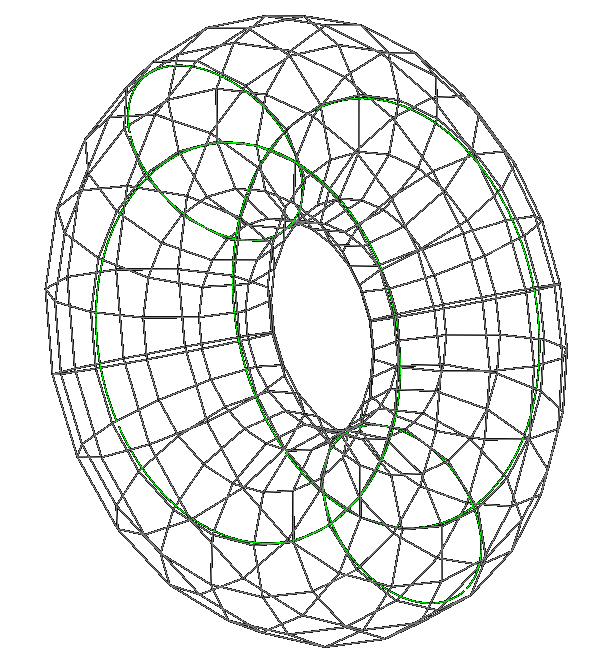
\includegraphics[width=0.5\textwidth]{Parameter_aligned_curves}
		\caption{Some Example Parameterization curves along the major axis of a torus. FIXME : Replace this with a better picture with thicker lines.}
		\label{fig:parameter_aligned_curves_torus}
		\end{figure}

	\subsection{Extracting the Morse-Smale Complex for the Visibility Function}
	
		// FIXME: I need to add some background information about the Morse-Smale Complex.
	We now have ridge sets and valley sets, which may be isolated points. We then procceed to union all disconnected sets together and add their levels to the final output.
		
		\begin{algorithm}
		\caption{For a given height $h$, finds exactly 1 point on every level set closed curved defined for a function $\mathbb{R} \times \mathbb{R} \rightarrow \mathbb{R}$ on a surface with no boundary that is morse,
			     i.e their critical points are non degenerate and seperate.}
		\label{alg:findAllUniqueLevelSets}
		\begin{algorithmic}
		\STATE	Find all minima, maxima, and saddle points.
				We will call these features.
				Note that it is possible to calculate the equivalence to two features,
				because we can follow the gradient to theoretically arbitrary precision.
				We assume in this problem that all features are isolated as in the definition of a morse function.
		\STATE	Connect every saddle point to its 2 neighboring maxima and 2 neighboring minima using gradient descent to follow the integral curves.
				Remember the locations on the level sets where they are intersected by the integral curves.
		\STATE     We now have a Morse-Smale complex?) that looks something like Figure : \ref{fig:MorseSmale}.
		\STATE	We will use a union find algorithm to separate G into disjoint regions that I will call ridges and valleys.
				A ridge is a connected set of features that are all above the level h.
				A valley is a connected set of features that are all below the level h.
		\STATE Initialize a Union Find Structure $UF$
		\STATE Make a singleton set for every initial feature. // FIXME : Replace the singleton word?
		\FOR{ $(c_{1}, c_{2}) \in Edges(G)$}
			\IF{$h \not \in [f(c_{1}, f(c_{2})]$}
				\STATE $UF$.union$(c_{1}, c_{2})$ Union sets together if they are they do not cross the $h$ level.
			\ENDIF
		\ENDFOR
// FIXME : I need to simplify the prose for this pseudo-code algorithm.
		\end{algorithmic}
		\end{algorithm}


\begin{figure}[h]
\centering
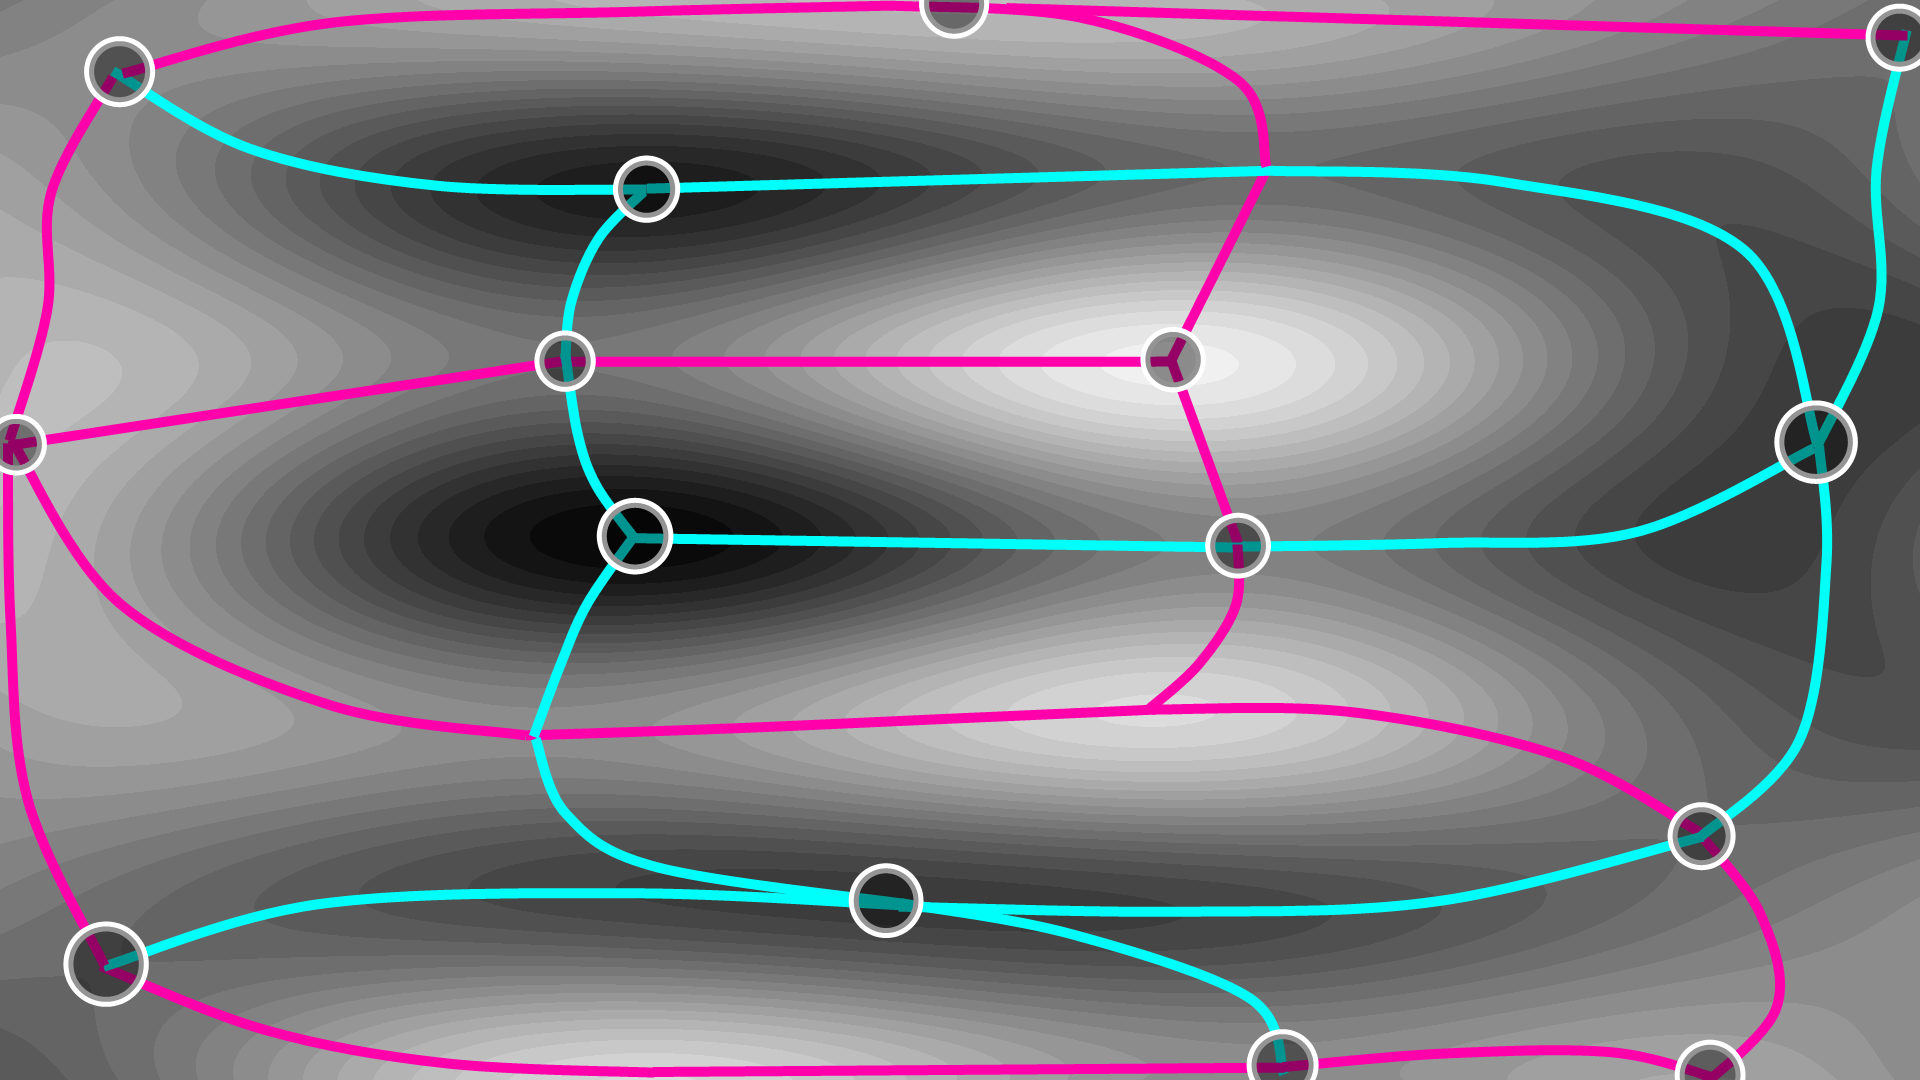
\includegraphics[width=0.5\textwidth]{minima_maxima_saddle_graph.png}
\caption{Morse Smale Complex of a function in two variables, i.e $\mathbb{R} \times \mathbb{R} \rightarrow \mathbb{R}$. Every saddle point connects to 2 minnima and 2 maxima.}
\label{fig:MorseSmale}
\end{figure}


	\subsection{Extracting Silhouette Curves}

		\subsubsection{Finding Exact representations of Silhouette Curves}
			// FIXME: Discuss finding roots of multinomial roots, and morse smale complex.
	
		\subsubsection{Curve Tracing Method}

			Because it is intractable to find the exact representations for silhouette curves, we use the practical curve tracing algorithm \ref{alg:TraceSilhouettes}.
			This algorithm is similar to the work of \cite{XJY98}.

			We find silhouette curves as follows:

			\begin{enumerate}
			\item Find all silhouette points that lie on patch boundaries. This may be acomplished via a 1D root finding algorithm in one parameter along the surfaces. 
				Please see section \ref{section:findingSilhouettePoints} for more information.
			\item Trace the curves
				Move in the direction perpendicular to the gradient of the function, then move back to the silhouette curve by optimizing the following function:
			$$\nabla f^{2}(u, v)$$ when doing the optimization, use appropiate step bounding as in Section \ref{section:GD}.
			\end{enumerate}

			%% Computes Silhouette Curves.
			\begin{algorithm}                      % enter the algorithm environment
			\caption{Given a surface, this algorithm computes a set of \textbf{sillhouette curve discretizations},
				each consisting of silhouette points and cooresponding tangent vectors pointing along the silhouette curve.
				We use an $\epsilon$ value of $.1$ which yields roughly $\frac{1}{\epsilon} = 10$ steps per patch, because each patch constitutes a 1 by 1 square in parameter space.} % give the algorithm a caption.
			\label{alg:TraceSilhouettes}       % and a label for \ref{} commands later in the document
			\begin{algorithmic}                    % enter the algorithmic environment
			    \REQUIRE The surface must be \textbf{continuous}, \textbf{differentiable}, and contain disjoint silhouette curves.
			    \ENSURE  If the surface has no boundaries, then the output curves are closed loops.
				\STATE \textbf{begin}
			    \STATE $S \Leftarrow $ Silhouette Point Finding Algorithm \ref{alg:FindSilhouettePoints}.
			    \FOR{ Point $p \in S$}
			        \STATE $(u_{0}, v_{0}) \leftarrow (p.u, p.v)$
				\STATE $(u, v) \leftarrow (u_{0}, v_{0})$
				\REPEAT
				        \STATE $(dv, -du) \leftarrow \nabla f(u,v)$
					\STATE normalize $(du, dv)$.
					\STATE $(u, v) \leftarrow (u, v) + \epsilon \cdot (du, dv)$
					\STATE $(u, v) \leftarrow $ GD $(\nabla(f^{2}),(u,v))$.
					\STATE Output point g(u, v) and tangent (du, dv).
				\UNTIL{$(u, v) == (u_{0}, v_{0})$}
			   \ENDFOR
				\STATE \textbf{end}
			\end{algorithmic}
			\end{algorithm}

			\begin{algorithm}                      % enter the algorithm environment.
			\caption{Given a surface, this algorithm finds the set of all silhouette points that lie on patch boundaries.} % give the algorithm a caption.
			\label{alg:FindSilhouettePoints}  % and a label for \ref{} commands later in the document.
			\begin{algorithmic}                    % enter the algorithmic environment.
			 	\REQUIRE The silhouette points on the boundaries need to be sufficiently far apart to prevent numerical instabilities.
				\ENSURE  
				\STATE \textbf{begin}
				\STATE $S \Leftarrow \emptyset$
				\FOR {$e \in Edges$}
					\STATE Compute the polynomial $p$ representing the silhouette function $f$ along $e$.
					\STATE Add all roots $\in [0, 1]$ of $p$ to $S$.
				\ENDFOR
			 	\STATE \textbf{return} $S$.
				\STATE \textbf{end}
			\end{algorithmic}
			\end{algorithm}

%			\begin{algorithm}                      % enter the algorithm environment.
%			\caption{Given a surface} % give the algorithm a caption.
%			\label{alg:FindSilhouettePoints}  % and a label for \ref{} commands later in the document.
%			\begin{algorithmic}                    % enter the algorithmic environment.
%			    \REQUIRE The surface must be \textbf{continuous}, \textbf{differentiable}, and contain disjoint silhouette curves.
%			    \ENSURE  If the surface has no boundaries, then the output curves are closed loops.
%			    \STATE Find at least 1 point on every silhouette curve. // FIXME: Quote algori
%			\end{algorithmic}
%			\end{algorithm}	


		\subsubsection{Finding Silhouette Points}
			\label{section:findingSilhouettePoints}

			// Discuss Morse Smale Algorithm.
			// Discuss our method and concerns over sampling.
			// Look up my description of the algorithm to Keenan.

			Because it is intractable to find the exact representations for sillhouette curves, we instead resort to finding a Silhouette points that 
			lie along the boundary of patches. Ideally we would like to only find one silhouette point per disjoint silhouette curve,
			which would elliminate the overhead of checking for curve equivalence,
			because otherwise we run the risk of tracing the same silhouette curves multiple times.



		\subsubsection{Finding Silhouette Points Via 1D Root Finding on Geometry Patches}
		\label{section:rootFindingGeometryPatch}

		To find the silhouette points along a boundary of a geometry patch, we first expand the definition of the visibility function as follows:

		$$ f = E \cdot (G_{u} \times G_{v}) $$
		$$ G_{u}(u, v) = \sum_{i=0}^{3} \sum_{j=0}^{3} \mathcal{B'}_{i}^{3}(u) \mathcal{B}_{j}^{3} (v) G_{i, j} $$
		$$ G_{v}(u, v) = \sum_{i=0}^{3} \sum_{j=0}^{3} \mathcal{B}_{i}^{3}(u)  \mathcal{B'}_{j}^{3} (v) G_{i, j} $$

		If we assume that u = 0, then we can simplify these partial derivatives as follows:

		\begin{equation} \label{eq:Pv0v}
		P_{u} = -3 \sum_{j=0}^{3} \mathcal{B}_{j}^{3}(v) G_{0, j} + 3 \sum_{j=0}^{3} \mathcal{B}_{j}^{3}(v) G_{1, j}
		\end{equation}
		\begin{equation} \label{eq:Pu0v}
		P_{v} = \sum_{j=0}^{3} \mathcal{B'}_{j}^{3} (v) G_{0, j}
		\end{equation}

		To compute the silhouette points along a boundary or any other 1 - dimensional axis aligned slice of a patch, evaluate the partial derivative with either $u$ or $v$ set to a constant value,
		 such as $u = 0$ in Equations \ref{eq:Pv0v} and \ref{eq:Pu0v}. This results in partials represented by 3-dimensional vectors containing single variable polynomials for each dimension.
		The visibility function polynomial may then be computed directly form the visibility function formula applying the cross product and dot product operations as
		as normal, but with polynomial algebra, instead of scalar algebra. The resulting single variable polynomial represents the value of the visibility function 
		along the given axis aligned slice within the input variable domain [0, 1].
		The roots of this polynomial coorespoind to Silhouette points. The roots may be computed using any single variable real root finding algorithm.
		We decided to implement root finding based on an interval bisection method using an interval counting method based on \emph{Sturm's theorem}\cite{AV10}, although numerical algorithms may have trouble discerning between roots that are sufficiently close to each other.
		They will also likely fail in the event of a silhouette curve runs along a boundary, because this will lead to an infinite number or roots.
		These Silhouette points work well, except when the silhouette curves cross boundaries between patches that contain extraordinary vertices.
		Please see Figure : \ref{fig:extraordinary_boundaries} for an example of the types of problematic behavior the extraordinary edges cause in our curve tracing algorithms.
		These problems provide the motivation for us to use tangent patches.

		\begin{figure}[h]
		\centering
		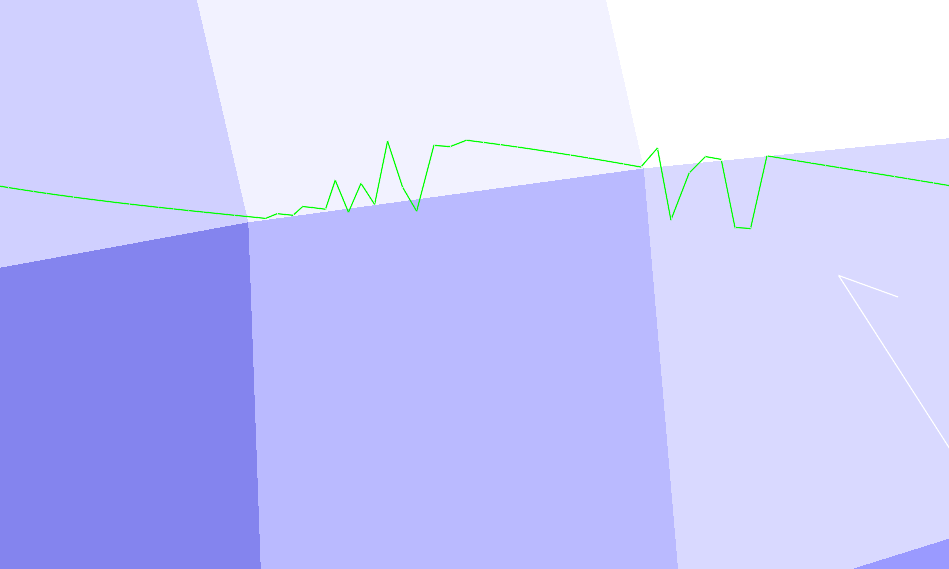
\includegraphics[width=0.5\textwidth]{ill_defined_silhouette_curves_over_extraordinary_boundary}
		\caption{Along extraordinary boundaries, the geometry patches are non differentiable and therefore the visibility function is discontinuous. This causes curve tracing to fail due to an invalidation of its assumptions.}
		\label{fig:extraordinary_boundaries}
		\end{figure}


		// FIXME : Should I call 'slices' something else.

		\subsubsection{Finding Silhouette Points Via 1D Root Finding on Tangent Patches}

		To compute the roots of the tangent patch defined visibility curve, please use Equations \ref{eq:g_u} and \ref{eq:g_v} for the partials.

		// FIXME : Should I discuss the tangent patches more?

		\subsubsection{Degenerate surface views}

		When a surface is oriented such that its silhouette curves are not disjoint, such as viewing a torus in a manner perfectly orthogonal to its hole.
		Please see Figure : \ref{fig:degenerate_torus_orientation} for an example near degenerate view of a torus.

		\begin{figure}[h]
		\centering
		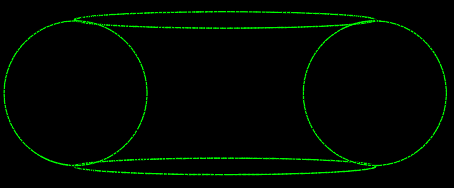
\includegraphics[width=0.5\textwidth]{torus_side_silhouettes}
		\caption{As a torus becomes oriented with its hole perpendicular to the vieing direction, its silhouette curves intersect each other. 
			This is one of several degenerate cases that present challenges to our curve tracing algorithms.}
		\label{fig:degenerate_torus_orientation}
		\end{figure}

		\subsubsection{Projecting 3D Discretizations onto 3D Planes}

		// FIXME : I need to discuss the conversion between 3D curves into 2D svg paths.

\section{Results}

We made a system that represents quadrilateral mesh defined Catmull-Clark subdivision surfaces through the the Loop-Shaeffer approximate via geometry and tangent patches.
We have developed some calculus for extracting curves on these surfaces, including the silhouette curves, parameter aligned curves, integral curves in
Morse-Smale complexes.
We have developed algorithms for finding the location of critical points for the Silhouette function \textbf{F}
Please see Figure: \ref{fig:pig_silhouettes} to see some extracted silhouette curves from a pig model.

Please see the following url for the research code that we wrote for this thesis: \url{https://github.com/Bryce-Summers/GeometricSurfaceCurves}.

\begin{figure}[h]
\centering
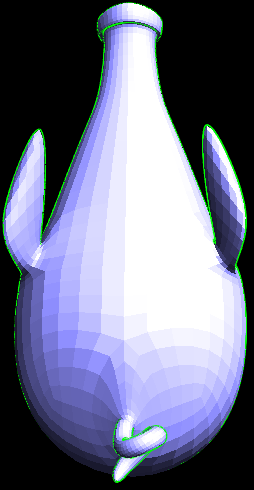
\includegraphics[width=0.25\textwidth]{Pig_patched}
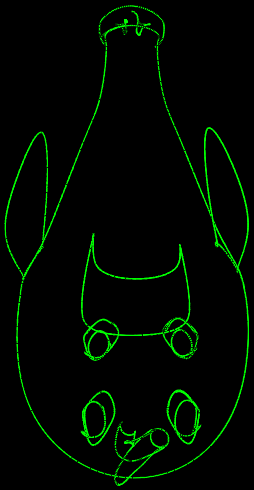
\includegraphics[width=0.25\textwidth]{Pig_silhouettes}
\caption{A view of a pig model rendered using Loop-Schaeffer geometry patches and some silhouette curves extracted via our system.
	The green curves on the right represent silhouette curves that we have extracted from the view of the pig model on the left and include curves that are
	occluded from our view, such as those surrounding the pig's four feet. There are some kinks and instabilities in these curves that should theoretically
	disappear once we use tangent patches instead of geometry patches.}
\label{fig:pig_silhouettes}
\end{figure}

\section{Comparison with prior work}

Past work including \cite{Eisemann08} has extracted silhouette curves from linear patches. They suffer from discontinuity and a lack of accurate interpolation of the points on the surface.
Please see Figure: \ref{fig:Eisemann_linear_patches} for an example of these problems. Please see Figure: \ref{fig:torus_silhouette_side_view} for an example silhouette curve that we extracted using our methods that is continuous everywhere and properly follows the surface.


\begin{figure}[h]
\centering
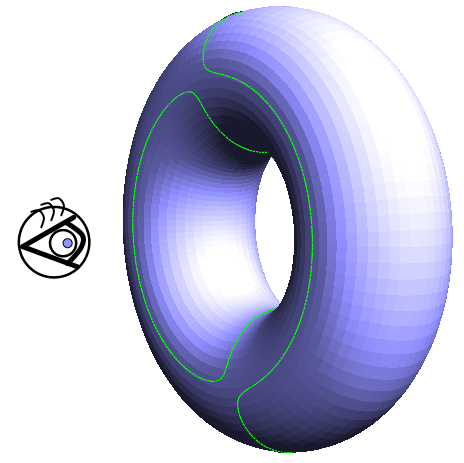
\includegraphics[width=0.5\textwidth]{torus_silhouettes_side_view}
\caption{Here are some silhouette curves extracted by our system that continuous even when not viewed by their defining viewing direction.
		The green curves represent the silhouettes generated from a viewing of surface from the left.}
\label{fig:torus_silhouette_side_view}
\end{figure}

\newpage

\section{Future Work}

Here we enumerate several problems that should be addressed in the future,
categorized into those that we feel can be immediatly tackled, those that may need to wait for mathematics to progress a bit,
and those whose realization is tied to the development of artifical intelligence.

	\subsection{Near Term Problems}

	In this section we will describe several coscisely stated problems similar to the silhouette curves problem that may be immediatly tackled in the near future.

		\paragraph{Extracting the Exterior Silhouette Curve.}
		The actual visual exterior for a surface may include subsets of several silhouette curves. The exterior silhouette curve may be computed by projecting the
		non-occluded silhouette curves onto the view plane as a planar graph embedding and extracting the exterior face.		

		\paragraph{Shadows.}
		We can compute direct shadows	by computing the exterior silhouette curves from a light source viewing in the direction of the surface and then projecting this exterior silhouette 
		onto a plane representing the ground that the surface is resting on. Since our silhouette tracing algorithm may be used to trace an arbitrary
		scalar function, we could also potentially compute the shadows cast by an object onto an arbitrary curved surface by composing the 
		visibility function of the shadow casting surface with the projection onto another surface to extract complicated shadows or even self-shadows.

		\paragraph{Minimum and Maximum Curvature Curves.}
		Minimum and maximum curvature curves may be used to communicate information about geometrically intuitive local coordinate systems in the neighborhood of specific points on an object.
		It would be very useful to be able to derive a 2D coordinate grid given a point on a surface.
	
		\paragraph{Geodesic Curves.}
		In the future, a user should be able to specify two points on a surface and receive the curve that represents the minimum distance path between those two points.
		This is known as the curve of minnimum geodesic distance.
	
		\paragraph{User Geometric Stylization Scheme.}
		Ideally, users could define a separation between geometric structure and the stylization applied to the geometry, much like cascading style sheets (CSS)
		define a seperation between content and style in the display of web pages today. 
		Users would be able to convert entire presentations, including the technical figures and imagery from one style to another automatically.
		A user should be able to define their own figure color scheme, label placement policy, viewing lighting and shadow orientations, etc in something like a CSS file and be able to automatically convert their figures between styles.

		\paragraph{Occlusion.}

		In our extracted curves, in addition to those points whose normals face away from the camera viewpoint,
		they may also include points that are not visible due to occlusion by other regions of the surface.
		There might be some interesting topological properties of closed curves that could be used for this task,
		especially if the homogenous depth of each of the points from the viewport was taken into account.
		
		\paragraph{Hot Wire Cutters.}

		Silhouette curves may be used to carve out surfaces without double negative curvature using hot wire cutters.
		There are some interesting problems related to this observation.

	\subsection{Medium Term Problems}

		In this section, we describe several problems that are more difficult,
		mainly because they involve geometric computations of a higher degree than the current mathematics of our day can handle.
		
		\paragraph{Perspective Correct Silhouette Curves.}
		Right now, we are assuming that the user is viewing the surface with an orthonormal view perspective where the eye is looking in one uniform direction.
		This approximation leads to visually acceptable silhouette curve computations, but it is not accurate in terms of the actual perspective projection that the figures are rendered in.
		To compute the curves in a perspective correct manner would require higher degree geometric computations .

		\paragraph{Extracting Exact Geometric Curves.}
		Right now we are extracting points and tangents along curves, but if people were to solve the problem determining the root curves of multinomials, then we could represent these curves without discretization.
		This is a difficult problem in algebraic geometry that is connected to other seemingly hard problems in computer science.

		\paragraph{Labeling Geometry.}

		It would be interesting to develop algorithms for properly placing textual labels for a given figure view where the labels are aware of the geometry.
		The labels placing would have to take into account desirable properties, such as avoiding overlapping lines, avoiding intersections with other labels, and encouraging visual orientation coherence, whereby the labels would all face roughly the same way.
		Arrows could also be investigated.

		\paragraph{2D Segmenting and Labelling Ray Traced Imagery.}

		A system could hypothetically be built that segments a 2D projection of a ray traced scene into different regions based on light transport phenomena.
		Please see Figure \ref{fig:cornell_box_illustration}.

		\begin{figure}[h]
		\centering
		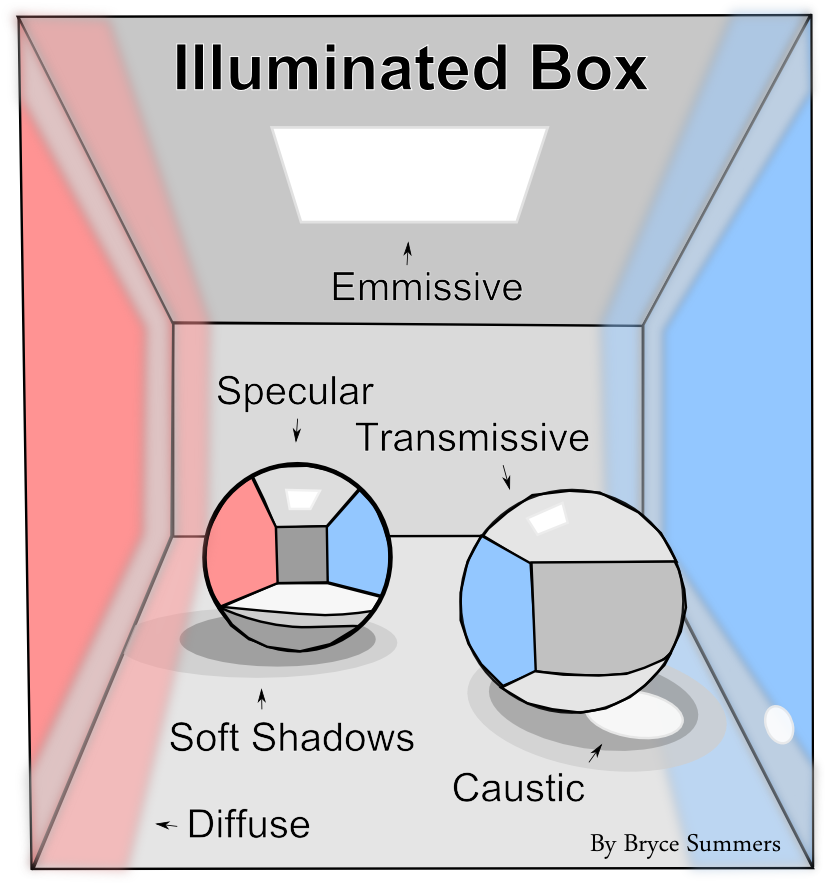
\includegraphics[width=0.5\textwidth]{cornell_box_illustration}
		\caption{A labeled illustration of the idea of converting a ray tracable scene into an SVG file with regions segmented by light transport phenomena.}
		\label{fig:cornell_box_illustration}
		\end{figure}


	\subsection{Long Term Problems}

		In this section, we will describe some long term grand problems that synthesize our work with Artificial Intelligence.

		\paragraph{Automatic Paper Interpretter.}
		In the future, a user could take a confusing research paper or any other work of communication feed it into a system and get a perfectly clear version of the paper back
		that even contains automatically generated illustrations of the ideas contined therin. This would enable us to reinterpret poorly written,
		poorly illustrated, or outdated papers in a form that is more readable and understandable for modern audiences and different types of learners.
		A person who shys away from mathematics or any other technical field because of the obtuseness of its academic literature would be able to 
		transform the writing into a more pallatable form.

\newpage

\begin{thebibliography}{9}

\bibitem{JDA08}
Tilke Judd, Frédo Durand, and Edward Adelson. 2007. 
\emph{Apparent ridges for line drawing}. ACM Trans. Graph. 26, 3, Article 19 (July 2007). DOI=http://dx.doi.org/10.1145/1276377.1276401

Elmar Eisemann, Holger Winnemöller, John C. Hart, and David Salesin. 2008.
\emph{Stylized vector art from 3D models with region support}. In Proceedings of the Nineteenth Eurographics conference on Rendering (EGSR '08). Eurographics Association, Aire-la-Ville, Switzerland, Switzerland, 1199-1207. DOI=http://dx.doi.org/10.1111/j.1467-8659.2008.01258.x

\bibitem{Eisemann08}
Elmar Eisemann, Holger Winnemöller, John C. Hart, and David Salesin. 2008.
\emph{Stylized vector art from 3D models with region support}. In Proceedings of the Nineteenth Eurographics conference on Rendering (EGSR '08). Eurographics Association, Aire-la-Ville, Switzerland, Switzerland, 1199-1207. DOI=http://dx.doi.org/10.1111/j.1467-8659.2008.01258.x

\bibitem{Catmull98}
E. Catmull and J. Clark. 1998. \emph{Recursively generated B-spline surfaces on arbitrary topological meshes.}
In Seminal graphics. ACM, New York, NY, USA 183-188. DOI=http://dx.doi.org/10.1145/280811.280992

\bibitem{Loop}
Charles Loop and Scott Schaefer. 2008.
\emph{Approximating Catmull-Clark subdivision surfaces with bicubic patches}.
ACM Trans. Graph. 27, 1, Article 8 (March 2008), 11 pages. DOI=http://dx.doi.org/10.1145/1330511.1330519

\bibitem{XJY98}
Li Xuejun, Sun Jiaguang, and Yang Changgui. 1998.
\emph{Extracting Silhouette Curves of NURBS Surfaces by Tracing Silhouette Points}.
Tsinghua Science and Technology. ISSN 1007-0214, 13/22, pp1005 - 1008, Volume 3, Number 2. (June 1998), 4 pages.

\bibitem{SEH08}
Matei Stroila, Elmar Eisemann, and John Hart. 2008.
\emph{Clip Art Rendering of Smooth Isosurfaces}.
IEEE Transactions on Visualization and Computer Graphics 14, 1 (January 2008), 135-145. DOI=http://dx.doi.org/10.1109/TVCG.2007.1058

\bibitem{AV10}
Akritas, Alkiviadis G., and Panagiotis S. Vigklas. 2010.
\emph{Counting the Number of Real Roots in an Interval with Vincent's Theorem}.
Bulletin Mathématique De La Société Des Sciences Mathématiques De Roumanie 53 (101) (3). Societatea de Științe Matematice din România: 201–211. http://www.jstor.org/stable/43679177.

\bibitem{other}
http://www2.cs.uh.edu/~chengu/Teaching/Spring2013/Lecs/Lec8.pdf



\end{thebibliography}

\newpage

\section{Apendix A: 3rd Order Bernstein Basis Functions and Derivatives.}

The Bernstein Basis functions of the third order are defined as follows:

$$B_{i} = \binom {3}{i} x^{i}(1 - x)^{3 - i}, \text{for} \; i \in \{0, \cdots, 3\}$$

Here is a listing of the four 3rd order bernstein polynomials along with their 1st, and 2nd order derivatives:

\begin{align*}
B_{0} &= (1 - x)^{3} \; & B_{0}' &= -3(1-x)^{2} \; & B_{0}'' &= - 6x + 6\\
B_{1} &= 3x(1 - x)^{2} \; & B_{1}' &= (x - 1)(9x - 3) \; & B_{1}'' &= 18 x - 12\\
B_{2} &= 3x^{2}(1 - x) \; & B_{2}' &= (6 - 9x)x \; & B_{2}'' &= -18x + 6 \\
B_{3} &= x^{3} \; & B_{3}' &= 3x^{2} \; & B_{3}'' &= 6x\\
\end{align*}

Here is a listing of the 3rd order bernstein polynomials in standard polynomial form along with their 1st derivatives in standard polynomial form:

\begin{align*}
B_{0} &= -x^{3} + 3x^{2} - 3x + 1 &B_{0}' &= -3x^{2} + 6x - 3\\
B_{1} &= 3x^{3} - 6x^{2} + 3x      &B_{1}' &= 9x^{2} - 12x + 3\\
B_{2} &= -3x^{3} + 3x^{2} &B_{2}' &= 9x^{2} + 6x\\
B_{3} &= x^{3} &B_{3}' &= 3x^{2}\\
\end{align*}

// FIXME: Consider putting a lovely picture here illustrating the Bernstein Polynomials.

\newpage

\section{Apendix B: 2nd Order Bernstein Basis Functions and Derivatives}

The Bernstein Basis functions of the third order are defined as follows:

$$B_{i} = \binom {2}{i} x^{i}(1 - x)^{2 - i}, \text{for} \; i \in \{0, \cdots, 2\}$$

Here is a listing of the 2nd order bernstein polynomials along with their 1st, and 2nd order derivatives:

\begin{align*}
B_{0} &= (1 - x)^{2} \;& B_{0}' &= 2x - 2 \; & B_{0}'' &= 2\\
B_{1} &= 2x(1-x) \;& B_{1}' &= -4x + 2 \; & B_{1}'' &= -4\\
B_{2} &= x^{2} \;& B_{2}' &= 2x \; & B_{2} &= 2\\
\end{align*}


Here is a listing of the three 2nd order bernstein polynomials in standard polynomial form along with their 1st derivatives in standard polynomial form:

\begin{align*}
B_{0} &= x^{2} - 2x + 1 \; & B_{0}' &= 2x - 2 \; & B_{0}'' &= 2\\
B_{1} &= -2x^{2} + 2x \; & B_{1}' &= -4x + 2 \; &B_{1}'' &= -4\\
B_{2} &= x^{2} \; & B_{2}' &= 2x \; &B_{2}'' &= 2\\
\end{align*}

// FIXME: Consider putting a lovely picture here illustrating the Bernstein Polynomials.

\newpage

%% Here is where I am putting a bunch of the large figures, which might inhibit the flow of the paper when they are placed inline.

\end{document}